\section{Introduction}
\pgfdeclareimage[width=1.0\paperwidth]{header-image}{header_images/fire2}


% Fire is important - why
% However, changes in fire are uncertain - fireMIP and Gittas paper.
% fireMIP
% JULES model type
% JULES performance
%  - best model of type
%  - best with prescribed veg
%  - veg model evaluation
%  - fire model evaultatrion
% Human fires
% Human suppression
%    From scores
%    From other studies
% Conclusions
% Slide to leave up: Other areas of fireMIP

% Slide 1: Burnt area; Areas of effected plants; Emissions; Radiative forcing
% Slide 2: FireMIP; Gittas model comp; Gittas benchmarking
% Slide 3: Firemip slide

\begin{frame}
	\frametitle{Fire In the Earth System}
	\framesubtitle{Areas affected}
	
	
	%\begin{textblock*}{14cm}(-0.5cm,1.5cm)
	%	\begin{tikzpicture}
		\only<1> {
			
			%\node[anchor=south west,inner sep=0] (image) at (0,0) {
				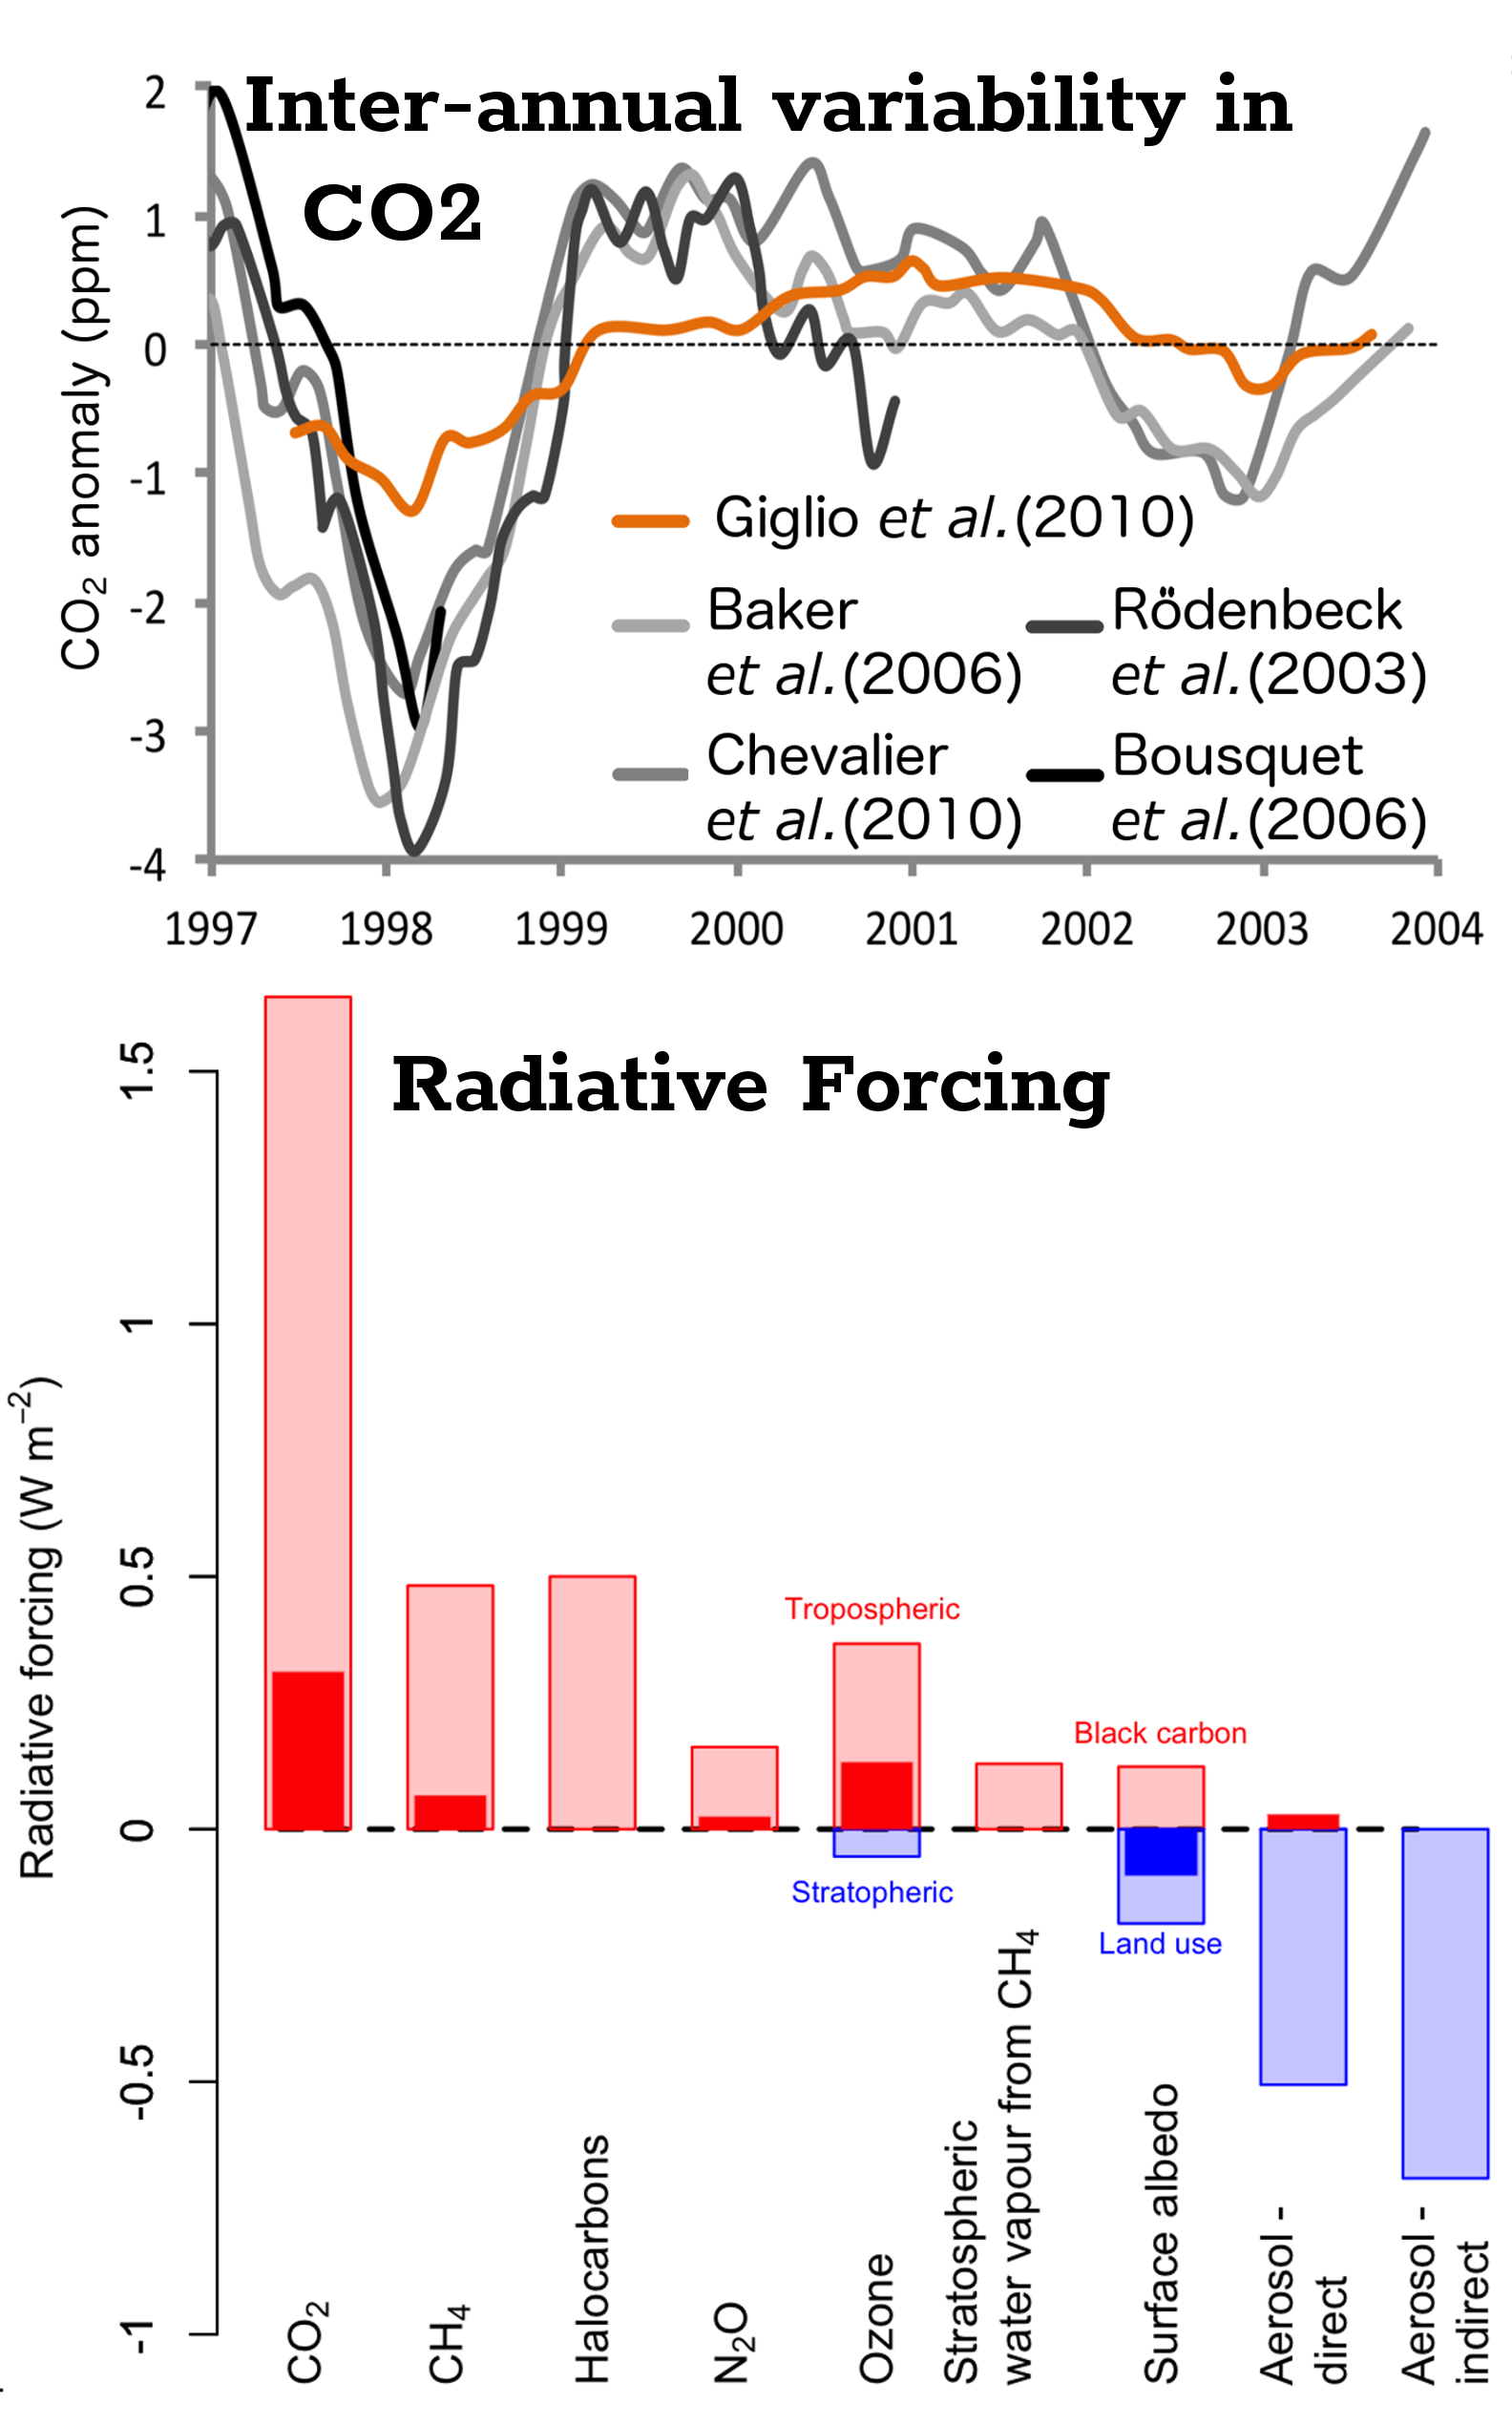
\includegraphics[width=10cm]{images/fireImportance}%images/unimodal/p\x.png}
			}%;}
		
		\only<2> {
			
			%\node[anchor=south west,inner sep=0] (image) at (0,0cm) {
				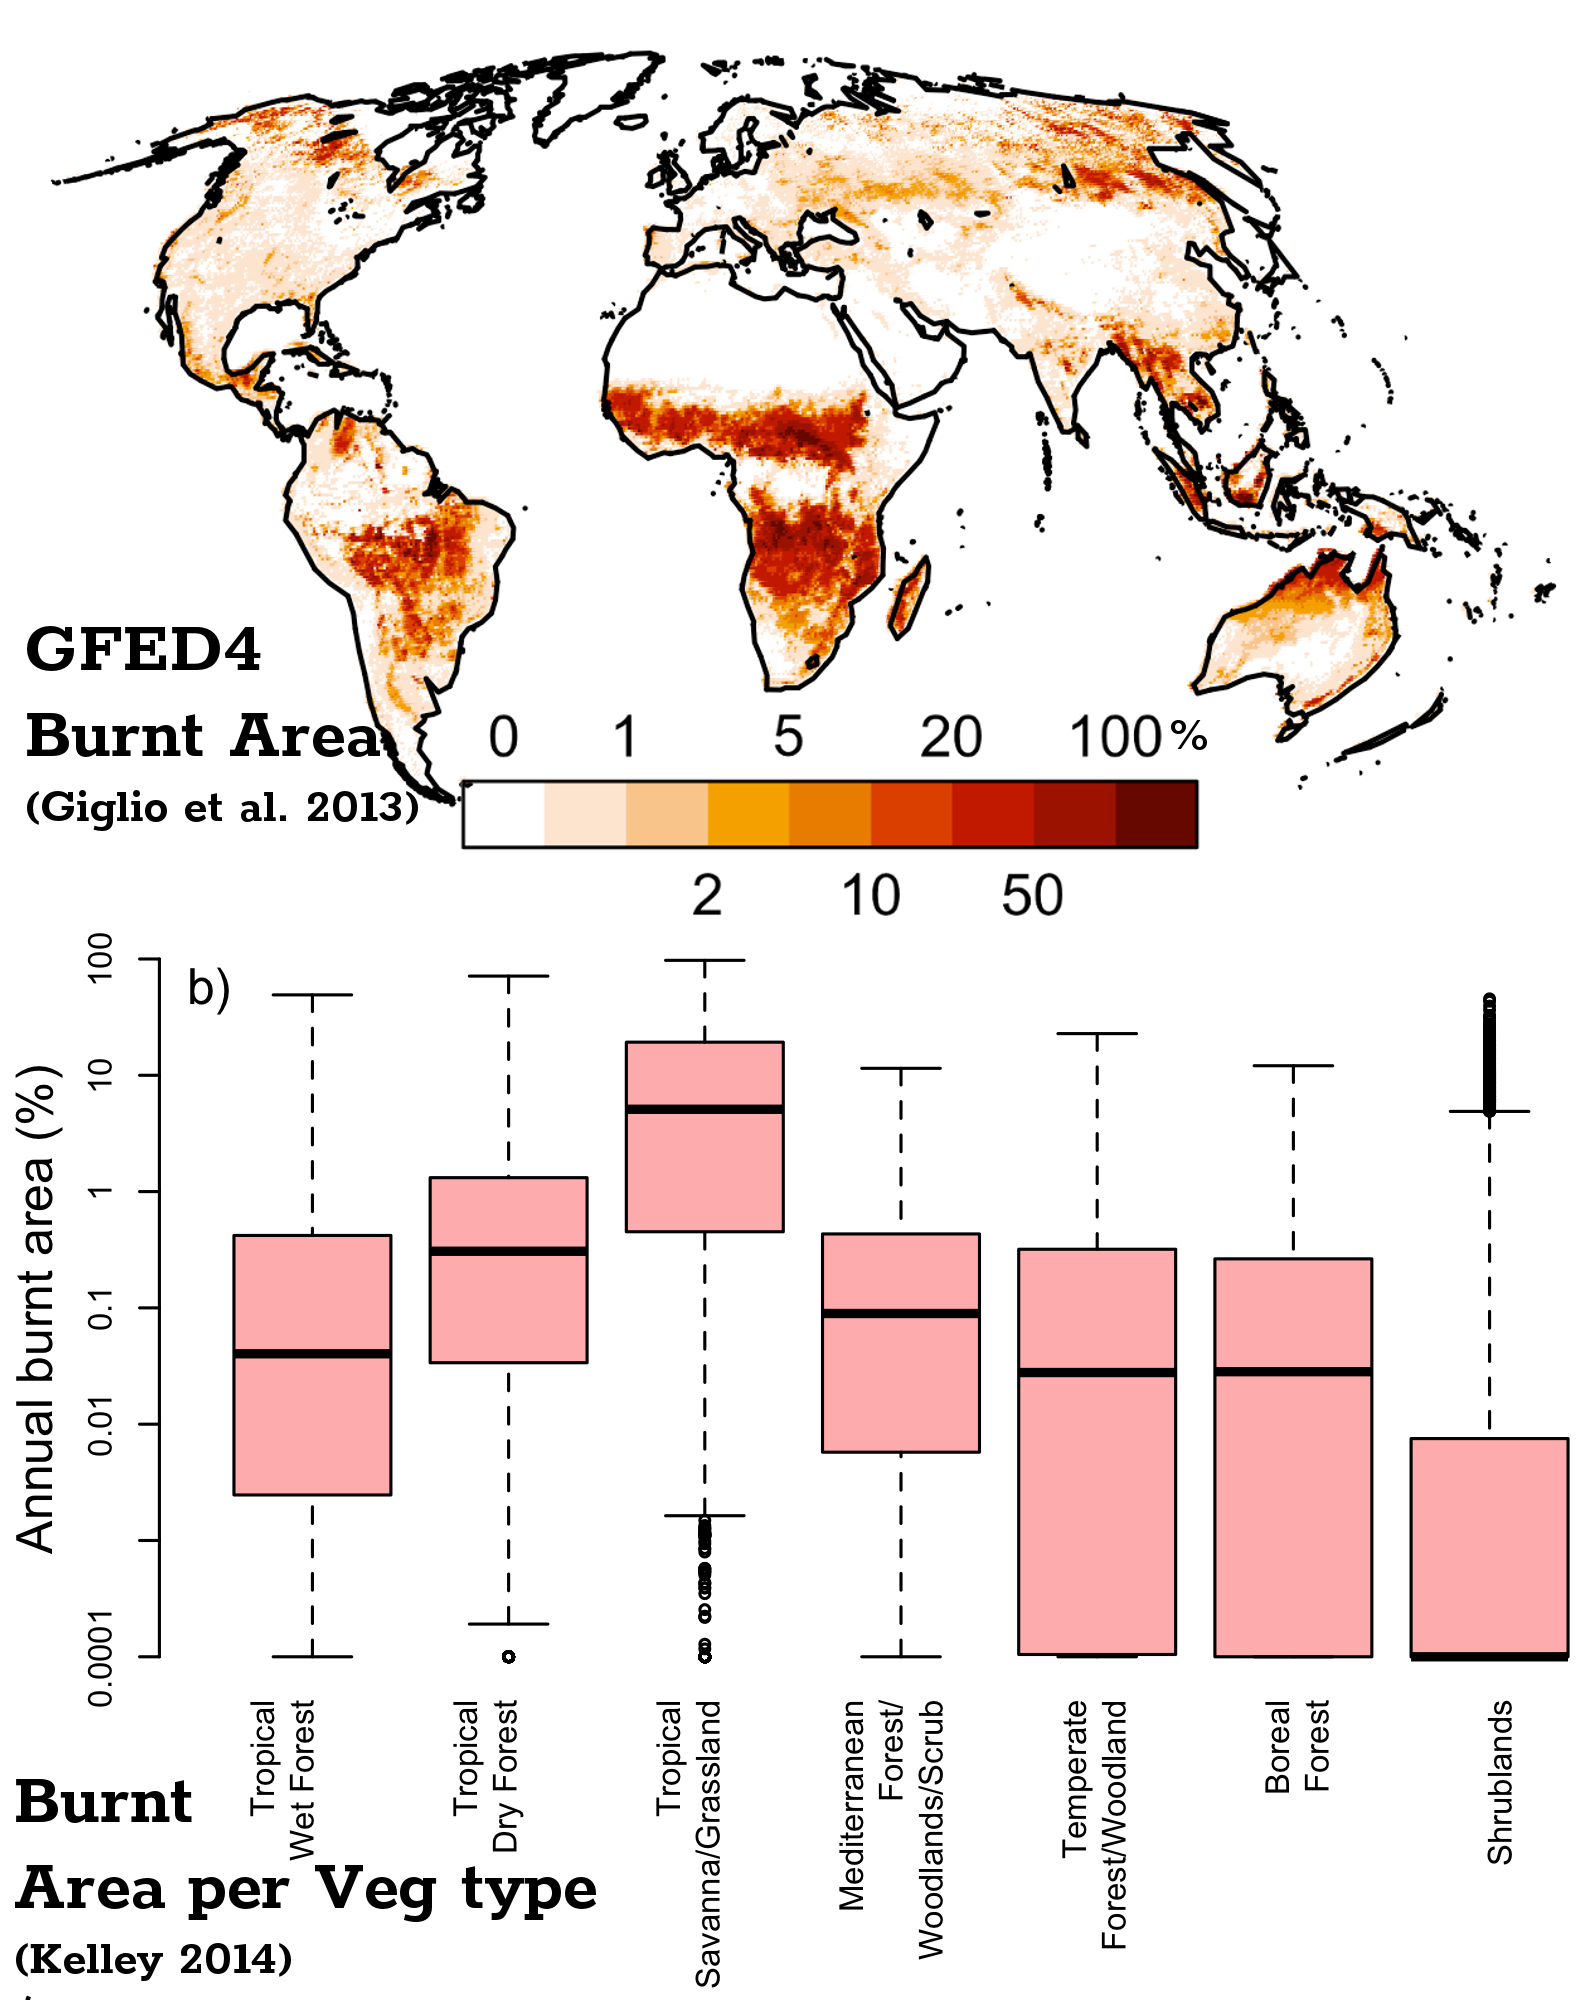
\includegraphics[width=10cm]{images/firePerBiome}%images/unimodal/p\x.png}
			}%;}
	%	\end{tikzpicture}
	%\end{textblock*}
	
	%Make clear we are talking about burnt area
\end{frame}



\begin{frame}[label = intro]
	\frametitle{What else controls fire?}
	%\framesubtitle{Is it Ignitions? Is it people?}
	\begin{itemize}
		\huge{
			\visible<1->{\item \hspace{2.39em}Is it ignitions?}
			\visible<2->{\item If so, Is it people or natural?}
			\visible<3->{\item \hspace{0.70em}Or, Is it something else?}
		}
	\end{itemize}
	\hspace{1.5cm} \only<4>{ (it's something else)}
	\visible<5->{(it's human suppression)}
	
\end{frame}


%\begin{frame}
%    \frametitle{What else controls fire?}
%    \framesubtitle{Fire-limitation framework}
%	\begin{itemize}
%		\visible<2-> {\item Map the limitation and sensitivity of burnt area to}
%        \begin{itemize}
%            \visible<3-> {\item Fuel discontinuity}
%            \visible<4-> {\item Fuel moisture and atmospheric drying potential}
%            \visible<5-> {\item lightning and human ignitions}
%            \visible<6-> {\item land use and human suppression}
%        \end{itemize}00
%		\visible<7-> {\item Controls are described from remote sensed and meteorological observations}
%		\visible<8-> {\item optimized againstburnt area observations}00
%	\end{itemize}
%\end{frame}
